\chapter{is}[is]

% avoiding spaces at the end of the author lines is not a problem with
% conference papers because we don't use \thanks or \IEEEmembership
% for over three affiliations, or if they all won't fit within the width
% of the page, use this alternative format:
%
%\author{\authorblockN{Michael Shell\authorrefmark{1},
%Homer Simpson\authorrefmark{2},
%James Kirk\authorrefmark{3},
%Montgomery Scott\authorrefmark{3} and
%Eldon Tyrell\authorrefmark{4}}
%\authorblockA{\authorrefmark{1}School of Electrical and Computer Engineering\\
%Georgia Institute of Technology,
%Atlanta, Georgia 30332--0250\\ Email: mshell@ece.gatech.edu}
%\authorblockA{\authorrefmark{2}Twentieth Century Fox, Springfield, USA\\
%Email: homer@thesimpsons.com}
%\authorblockA{\authorrefmark{3}Starfleet Academy, San Francisco, California 96678-2391\\
%Telephone: (800) 555--1212, Fax: (888) 555--1212}
%\authorblockA{\authorrefmark{4}Tyrell Inc., 123 Replicant Street, Los Angeles, California 90210--4321}}


% make the title area


\begin{abstract}
We present an importance sampling method for the evaluation of the low
frame error rate (FER) performance of LDPC codes under iterative
decoding.  It relies on a combinatorial characterization of absorbing
sets, which are the dominant cause of decoder failure in the low FER
region.  The biased density in the importance sampling scheme is a
mean-shifted version of the original Gaussian density, which is
suitably centered between a codeword and a dominant absorbing set.
This choice of biased density yields an unbiased estimator for the FER
with a variance lower by several orders of magnitude than the standard
Monte Carlo estimator.  Using this importance sampling scheme in
software, we obtain good agreement with the experimental results
obtained from a fast hardware emulator of the decoder.
\end{abstract}


\section{Introduction}

Low-density parity check (LDPC) codes are a class of binary linear
codes defined by very sparse factor graphs that yield excellent
error-correction performance when decoded iteratively using message
passing algorithms. Density evolution~\cite{richurbanke} accurately
characterizes their performance for large blocklengths.  However, for
moderate blocklengths---i.e., those on the order of hundreds to
thousands---the density evolution method can yield inaccurate results,
and thus current understanding of the finite length LDPC codes remains
incomplete.  In this moderate blocklength regime, many structured LDPC
codes exhibit an \emph{error floor}, corresponding to a significant
flattening in the curve that relates signal to noise ratio (SNR) to
the frame error rate (FER).  Consequently, despite the appeal of these
codes for many high data rate communications and data storage
applications, their wide-scale deployment has been hindered by
incomplete understanding of finite-length effects and error floors.
Better understanding of the performance of finite-length LDPC codes in
the low BER/FER regime has both theoretical as well as practical
implications. From a theoretical standpoint, it provides a deeper
understanding of the convergence of the message passing
algorithms. For practical storage and wireline applications, such
predictions provide a useful engineering tool in estimating performance
and designing LDPC codes.

Error-floor behavior can be attributed to the suboptimal nature of the
message passing algorithms used for decoding LDPC codes.  In early
work on error floors of LDPC codes, MacKay and Postol~\cite{mackay}
introduced the notion of a near-codeword.  Other related notions
include trapping sets~\cite{richardson},
pseudocodewords~\cite{Frey98}, and elementary trapping sets
\cite{milenkov}.  Based on our previous work~\cite{zhang06} using a
hardware emulator to explore the low FER region, we have isolated a
class of combinatorial structures that cause the decoder to fail by
converging to a non-codeword state. Due to their attractive nature, we
refer to these structures as \textit{absorbing sets}.  These
structures have a purely combinatorial definition in terms of the
parity check matrix defining the code, and can also be understood as a
particular type of near codeword~\cite{mackay} that is guaranteed to
be stable under a bit-flipping algorithm. For many LDPC codes, the
associated factor graphs contain absorbing sets which have strictly
fewer bits than the minimum codeword weight. As a result, the
performance of the decoding algorithm in the low FER region is
predominantly dictated by the number and the structure of minimal
absorbing sets, rather than the minimum distance
codewords~\cite{icc-theory}, as in the case of a maximum-likelihood
decoder.


In this paper, we investigate the low FER performance of a
$(2048,1723)$ Reed-Solomon based LDPC codes~\cite{rs-ldpc} as a
representative example of high-performance LDPC codes for which the
low FER region is dominated by non-codewords.  This particular RS-LDPC
code has been adopted in recent standards, and has a number of
desirable properties.  In this paper, we develop and demonstrate the
effectiveness of a fast simulation method, based on importance
sampling~\cite{Bucklew90}, for approximating the error probability.
As we discuss in more detail below, early work by
Richardson~\cite{richardson} demonstrated the effectiveness of a
two-stage approach, based on a combination of hardware emulation and
software-based simulation, for approximating the error probability.
Other work~\cite{ryan,ucla} has directly applied importance sampling
(IS), though limited to shorter blocklength codes and higher FERs than
those considered here.  For the RS-LDPC code, we first show how it is
possible to exactly enumerate all relevant classes of absorbing sets
that are dominant in the low FER regime.  We then exploit this
characterization of these absorbing sets to develop an efficient IS
method for evaluating the probability of error in the low FER regime.
The agreement with the experimental results obtained from the hardware
emulator demonstrates the power of the proposed technique, and
suggests that performance evaluation using the importance sampling
methods at even lower BER/FER levels yields reasonable
predictions. The computational advantage of the importance sampling
methods is demonstrated via their relative efficiencies--- namely, the
reduction in the sample variance of our IS-based estimators relative
to the sample variance of a naive Monte Carlo estimators, which
exceeds tens of millions.
%We also provide some new insight into the
%decoding regions around codewords and around absorbing sets, and we
%discuss how these regions change as a function of the decoder
%implementation.

The first paper (that we are aware of) that proposed a method for
predicting deep BER behavior of message-passing decoding algorithms is
by Richardson~\cite{richardson}.  This method consisted of two stages:
first identifying a class of (empirically defined) trapping sets via
hardware emulation, and then approximating its associated error
probability by simulating over a sequence of channel noises biased
towards the individual trapping set.  In contrast, our work is based
on graph substructures that have a combinatorial characterization in
terms of the Tanner graph, which we refer to as absorbing sets.  We
then approximate the error probability associated with a given
absorbing set by performing importance sampling at a single
mean-shifted distribution.  Our approach thus obviates the need to
empirically identify candidate trapping sets. While we may in theory
miss some error events through this approach, our simulation results
show sufficiently close agreement to our hardware emulations to argue
for the value of our approach.

 The remainder of the paper is organized as follows. In
Section~\ref{ldpcback}, we provide background on Reed-Solomon based
LDPC codes and absorbing sets.  Section~\ref{isback} describes the
Monte Carlo and importance sampling methods, and the specific IS-based
estimator used in this work.  Section~\ref{analysis} contains results
of the low FER rate performance using importance sampling. Lastly,
Section~\ref{conc} summarizes the results and proposes future
extensions.

%\vspace{1in}
\section{Background}

\label{ldpcback}

We begin with background on RS-LDPC codes, as well as on the notion
of absorbing sets.


\subsection{RS-LDPC codes}
Reed-Solomon based LDPC codes (RS-LDPC)~\cite{rs-ldpc} are regular,
structured LDPC codes, with the girth being at least 6.  The parity
check matrix of this code family can be viewed as consisting of a
two-dimensional array of permutation matrices of equal size. For the
row degree $\rho$ and the column degree $\gamma$, the construction is
based on stacking up $\gamma$ cosets of a one-dimensional subcode that
is itself determined by a weight $\rho$ codeword of a dimension 2
shortened Reed-Solomon code, followed by appropriately mapping these
symbols into binary row vectors. For the details of the construction,
please see Section III in the paper~\cite{rs-ldpc}.

The focus of this paper is the (2048,1723) RS-LDPC code, which has
column degree 6, row degree 32, and each component permutation
submatrix is of size 64 $\times$ 64.  This particular RS-LDPC has been
adopted in the IEEE 802.3an 10GBASE-T standard. The standard supports
10 Gb/s Ethernet over 100 meters of CAT-6a UTP (unshielded
twisted-pair) cable. The high frequency transmission is severely
impaired by insertion loss, cross talk, and interferences due to the
cable channel. These challenges present a stringent requirement on the
performance of the transceiver design. The $(2048,1723)$ RS-LDPC code
is selected specifically to provide sufficient coding gain to allow
for a bit error rate (BER) performance of $10^{-12}$ or
better~\cite{802standard}.  This code is designed to contain no cycles
of length 4 in the associated Tanner graph. It also features a
structured parity check matrix, amenable for a high throughput,
parallel decoder implementation. A lower bound on the the minimum
distance of this code is 8 by construction, though the actual minimum
distance is believed to be much higher. However, in our previous
hardware-based emulations~\cite{zhang06}, all error events recorded in
the low FER region were due to \emph{non-codeword} configurations.
More specifically, the decoder never converged to a non transmitted
codeword.  and all recorded errors were caused a single class of
combinatorial substructures.




\subsection{Absorbing sets}
As established in our previous experimental and theoretical
work~\cite{zhang06,icc-theory}, certain structures in the Tanner graph
associated with a parity check matrix of an LDPC code cause the
decoder to converge to a non-codeword state. We termed these
structures \emph{absorbing sets}, which are defined more formally as
follows:

\begin{figure}
%\vspace{0.1in}\hspace{0.2in}
%
\center
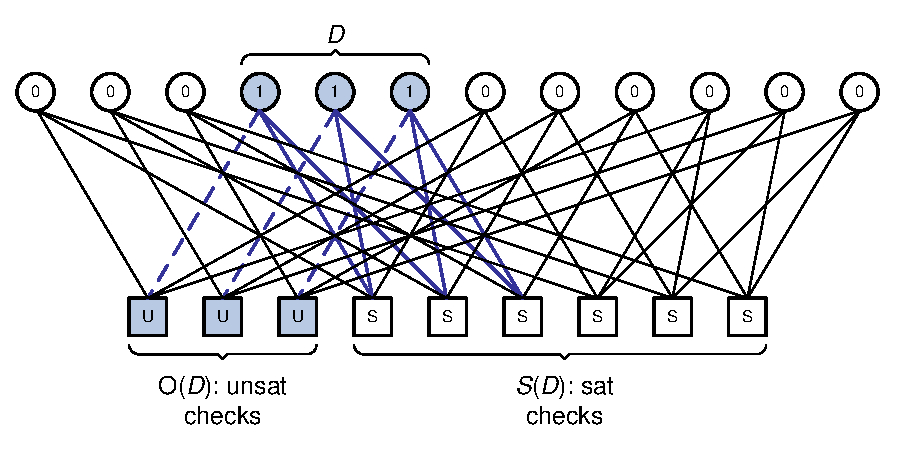
\includegraphics[width=3.2in,height=1.6in]{ITW07_33.eps}
%
\caption{An example of a (3,3) absorbing set.} \label{abs44}
\end{figure}

\vspace{0.0in}Let $G=(V,F,E)$ be a bipartite graph with the vertex
set $V \cup F$, where $V$ and $F$ are disjoint, and with the edge
set $E$, such that there exists an edge $e(i,j) \in E$ if and only
if $i\in V$ and $j\in F$.  One can associate a bipartite graph
$G_H=(V,F,E)$ with a parity check matrix $H$, such that the set $V$
corresponds to the columns of $H$, the set $F$ corresponds to the
rows of $H$, and $E=\{ e(i,j)| H(j,i)=1\}$. Such a graph $G_H$ is
commonly referred to as the Tanner graph of the parity check matrix
$H$ of a code. Elements of $V$ are called ``bit nodes'' and elements
of $F$ are called ``check nodes''. For the subset $D$ of $V$ we let
$N_D$ denote the set of check nodes neighboring the elements of $D$.

For a subset $D$ of $V$, let $\mathcal{E}(D)$ (resp.
$\mathcal{O}(D)$) be the set of neighboring vertices of $D$ in $F$
in the graph $G$ with even (resp. odd) degree with respect to $D$.
Given an integer pair $(a,b)$, an $(a,b)$ \emph{absorbing set} is
a subset $D$ of $V$ of size $a$, with $\mathcal{O}(D)$ of size $b$
and with the property that each element of $D$ has strictly fewer
neighbors in $\mathcal{O}(D)$ than in $F\backslash
\mathcal{O}(D)$. We say that an $(a,b)$ absorbing set $D$ is an
$(a,b)$ \emph{fully absorbing set}, if in addition, all bit nodes
in $V\backslash D$ have strictly more neighbors in $F\backslash
\mathcal{O}(D)$ than in $\mathcal{O}(D)$ \cite{icc-theory}.


Thus, absorbing sets correspond to a particular type of near-codeword,
distinguished by the additional requirement of each bit having
strictly more satisfied than unsatisfied checks.  An example of an
$(a,b)$ fully absorbing set with $a=b=3$ is given in Fig.~\ref{abs44}.
For the (2048, 1723) RS-LDPC code, the dominant (fully) absorbing sets
are (8,8) absorbing sets. An example of such a configuration is given
in Figure 2. The bits outside of the (fully) absorbing sets, though
omitted from the figure for clarity, are also assumed to have strictly
more satisfied than unsatisfied checks.


%\onecolumn
\begin{figure*}
\vspace{0.0in}\hspace{0.4in}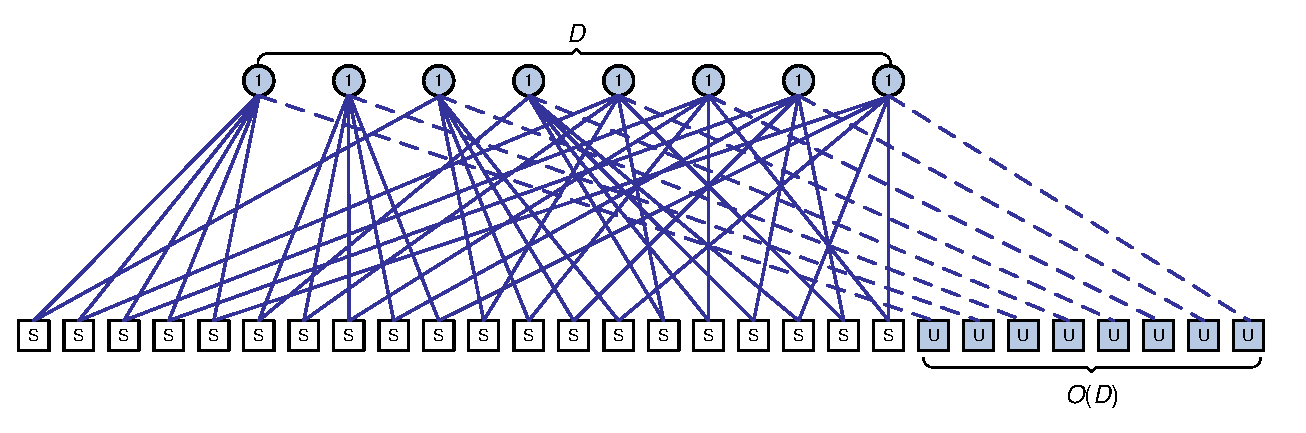
\includegraphics[width=5.4in,height=1.7in]{ITW07_88.eps}
\caption{An example of a (8,8) absorbing set for the $(2048,1723)$
RS-LDPC code.  Each of the $8$ bits in the set are connected to $4$
satisfied checks, and $1$ unsatisfied check.  } \label{abs88}
\end{figure*}
%\twocolumn





%\vspace{1in}


\vspace{0in}\section{Monte Carlo and Importance Sampling}
\label{isback}

Suitably designed LDPC codes of moderate blocklength yield excellent
performance when decoded with suboptimal iterative message-passing
algorithms.  The performance of an iteratively decoded LDPC code is
typically reported as the (empirical) probability of error for a
certain SNR value. For high SNR values, this empirical probability is
very small and thus a large number of trials needs to be executed in
order to estimate it reliably.

\subsection{Some intuition}

To provide some intuition for the typical number of samples required,
suppose that $p$ is the true probability of a decoding error at a
certain SNR level. A naive Monte Carlo simulation entails running the
decoder on $N$ independent channel realizations, and recording the
output of each trial $i= 1, \ldots, N$ with a Bernoulli indicator
variable
\begin{eqnarray*}
Z_i & \defn & \begin{cases} 1 & \mbox{if decoder fails on trial $i$} \\
                         0 & \mbox{otherwise.}
       \end{cases}
\end{eqnarray*}
It is assumed that the decoding error in the $i^\text{th}$ trial
occurs whenever the decoder does not converge to the transmitted
codeword in the fixed number of iterations.  These Bernoulli indicator
variables then yield the naive Monte Carlo estimate
\begin{eqnarray}
\label{EqnNaiveMC}
\hat{p}_{MC} & \defn & \frac{1}{N}\sum_{i=1}^N Z_i.
\end{eqnarray}
The Monte Carlo estimator is unbiased and has variance
$\var(\hat{p}_{MC})=\frac{1}{N}\left(\hat{p}_{MC}-\hat{p}_{MC}^2\right)$.

In order to characterize the quality of $\hat{p}_{MC}$ as an estimator
of $p$, we require that the relative error be small with high
probability, or equivalently that the tail probability
\begin{equation}
\label{EqnTail}
\mathbb{P} \left[ \left|\frac{\hat{p}_{MC}-p}{p}\right| > \epsilon
\right]
\end{equation}
should be small for an appropriate $\epsilon > 0$.  Some algebra
yields that
\begin{eqnarray*}
\mathbb{P} \left[ \left|\frac{\hat{p}_{MC}-p}{p}\right| > \epsilon
\right] & = & \mathbb{P} \left[ \frac{1}{N}\sum_{i=1}^N
\frac{Z_i-p}{\sqrt{p \,(1-p)}}> \epsilon \sqrt{\frac{p}{1-p}} \right].
\end{eqnarray*}
Since $Z_i$, $1 \leq i \leq N$ are i.i.d. Bernoulli random variables,
we may invoke the central limit theorem to approximate this
probability as the Gaussian tail function $\mathbb{P} [\left| Y
\right| > y]$, where $Y$ is a standard normal random variable and
\mbox{$y= \epsilon \sqrt{N \, p/(1-p)}$.}  As a concrete example, if
we require that for tolerance $\epsilon = 0.2$ the tail
probability~\eqref{EqnTail} be at most 0.05, corresponding to a 95\%
confidence interval, then we need $y \approx 2$, and thus $N \approx
100 (1-p)/p$. Consequently, in order to estimate a probability of
error that is around $10^{-8}$ up to relative error $\epsilon = 0.2$,
on the order of $10^{10}$ trials are needed. Such a requirement poses
a significant computational burden on available resources.


\begin{figure}\centering
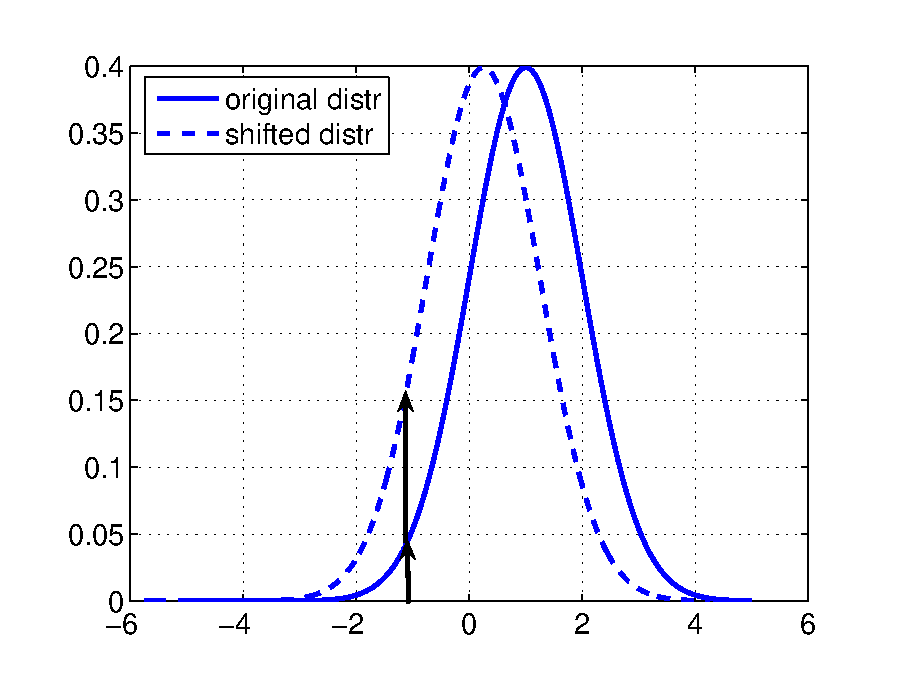
\includegraphics[width=2.4in,keepaspectratio]{itwfig3a_lara3.eps}
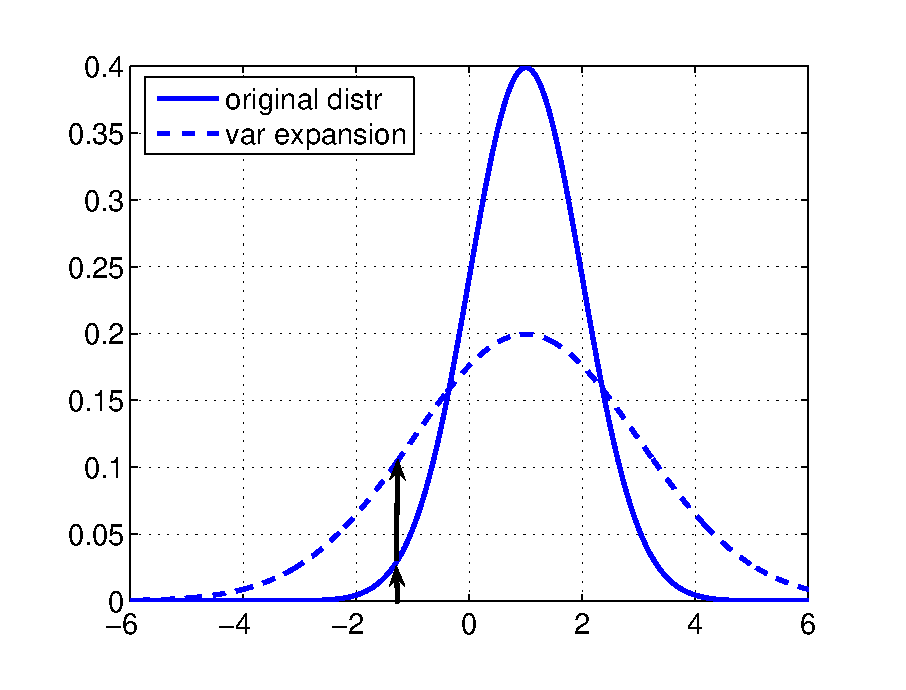
\includegraphics[width=2.4in,keepaspectratio]{itwfig3b_lara3.eps}
\caption{Examples of biasing densities (top: mean shift, bottom:
variance increase).} \label{bias}
\end{figure}

 The motivation underlying importance sampling is to appropriately
modify the original density such that the infrequent errors become
more likely. For a Gaussian density one may choose to shift the mean
or to scale the variance, as shown in the top and bottom panels of
Figure~\ref{bias} respectively.  In both cases the probability of the
event in the tail part (marked with an upward arrow in the Figures) of
the original distribution significantly increases.  The biasing
density should be chosen in such a way that the variance associated
with its estimator provides a substantial improvement over the
variance of a naive Monte Carlo estimator. Specifically, the ratio of
these two quantities indicates the reduction in the number of trials
needed to achieve the same confidence of the estimate of the
probability of error.

Supposing that one draws samples according to the biasing density
$f_{bias}$ instead of the original density, the importance sampling
estimator is computed as
\begin{eqnarray}
\label{EqnDefnIS}
\hat{p}_{IS} & = & \frac{1}{N}\sum_{i=1}^N Z_i w_i,
\end{eqnarray}
where the \emph{importance sampling weight} $w(x_i)
=f(x_i)/f_{bias}(x_i)$ reweights the contribution of the $i^{th}$
trial so that the estimator is unbiased ($\mathbb{E}[\hat{p}_{IS}] = p$).
Moreover, the IS variance is given by
\begin{eqnarray*}
\var(\hat{p}_{IS})=\frac{1}{N} \left( \frac{1}{N} \sum_{i=1}^N
\left(Z_i w_i \right)^2 -\hat{p}_{IS}^2 \right).
\end{eqnarray*}


\subsection{Error probabilities via mean-shifted importance sampling}

We propose to employ a biasing density $f_{bias}$ that makes the
decoder converge to an absorbing set more frequently.  As observed in
our previous work~\cite{zhang06} on the $(2048,1723)$ RS-LDPC code,
all errors in the low BER region are due to the absorbing sets of the
$(8,8)$ type.  We are concerned with the transmission over an AWGN
channel using BPSK modulation with mapping $0 \rightarrow +1$ and $1
\rightarrow -1$. Due to symmetry, we assume that the all-zeros
codeword is transmitted.  We choose $f_{bias}$ to be a mean-shifted
version of the original density $f$, which (assuming that the
all-zeroes codeword was transmitted) is a Gaussian density with mean
$[1 \; 1 \dots 1]$ and the variance $\sigma^2 I_{n \times n}$.  Since
$(8,8)$ absorbing sets dominate the low FER region, we set the mean
shift to be $\meanshift$ in the bits belonging to a particular $(8,8)$
absorbing set, and zero for the remaining bits.  As a result, the
importance sampling reweighting function $w(\cdot)$ takes the form
\begin{eqnarray}
\label{EqnDefnWeight} w(x; \meanshift, \sigma^2) & \defn &
\frac{e^{-\frac{1}{2 \sigma^2} \left[\sum_{j=1}^8 (x_{k_j}-1)^2
\right]}} {e^{-\frac{1}{2 \sigma^2} \left[\sum_{j=1}^8
(x_{k_j}-(1-\meanshift))^2\right]}}
\end{eqnarray}
where $k_1$ through $k_8$ are indices of the $8$ bits participating in
the $(8,8)$ absorbing set.

Importance sampling is most effective when the density is neither
underbiased nor overbiased, meaning that a reasonable choice for the
mean-shift $\meanshift$ is one which causes the decoder to return the
correct all-zeros codeword and to the targeted $(8,8)$ absorbing sets
with roughly equal probability.  In our work, we empirically
determined this point is chosen to be roughly $\meanshift = 1.2$. Note
that the contrast with maximum likelihood decoding where $\meanshift =
1$ defines the hyperplane separating decoding regions of two competing
codewords. Figure~\ref{tab1} lists the ratio of the decoding errors
over the total number of trials for different mean shifts. When the
total number of trials is fixed and relatively low, choosing the mean
shift value of $\meanshift = 0.8$ or less produces very infrequent
decoding errors. Likewise, for the the mean shift of $\meanshift =
1.6$ or higher, the decoder almost always makes an error, and coupled
with very low weighting terms $w(x)$ uniformly underestimates the
probability of error. For the middle region where $\meanshift$ is
between $1.0$ and $1.4$, the simulation results described in the next
section changed only negligibly with $\meanshift$.

%\vspace{0in} MISSING POINT 2: DISCUSSION OF MEAN SHIFT WRT
%VARIANCE.




\begin{figure}\center\begin{tabular}{|c|c|c|c|c|}
  \hline
  % after \\: \hline or \cline{col1-col2} \cline{col3-col4} ...
  Mean Shift & Ratio  \\
  \hline
  0.8 & 0.0134  \\
  1.0 & 0.1712  \\
  1.2 & 0.6292  \\
  1.6 & 0.9976  \\
  1.8 & 0.9999  \\
  \hline
\end{tabular}
\caption{Ratio of absorbing set errors and total number of trials
for the 6-bit decoder.}\label{tab1}
\end{figure}

%\begin{figure}
%\includegraphics[width=2.8in,height=1.6in]{Drawing1.ps}
%\caption{Illustration of the decoding region. } \label{decRegion}
%\end{figure}
%As illustrated in Figure~\ref{decRegion},
%The decoding region around a codeword is postulated to be larger than
%around a neighboring absorbing set.

Consider the set $S$ of the bit nodes in which the codeword and the
neighboring absorbing set disagree, and which participate in
unsatisfied checks in this absorbing set. Since the decoder aims to
have all checks satisfied, the values at these nodes in $S$ would have
to be strongly incorrect, i.e. close to the absorbing set in the
$n$-dimensional space, for their values not to be overcome by the
neighboring unsatisfied checks. The more of the unsatisfied checks
there are in the absorbing set, the smaller the decoding region of
that set is, since the values associated with the elements of $S$ need
to be reasonably close to the absorbing set values to resist the
messages sent from a large set of unsatisfied checks. Since for the
(8,8) set, there is one unsatisfied check per the bit node in the
absorbing set out of the total of 6 neighboring checks, the relative
size of the decoding region around this absorbing set is then somewhat
smaller than the one associated with the nearest codeword in the
direction of the coordinate which has value 0 for the codeword and 1
for the absorbing set.

While a variance-scaled Gaussian (see Fig.~\ref{bias}) may also be
considered as a candidate biasing density, choosing this density does
not lead to satisfactory results.  For smaller variance scalings, the
relative number of observed errors is quite small, so that a much
larger number of trials are required for estimates of accuracy
comparable to the mean-shifted estimator.
%in order to prevent extreme underestimation of the probability of
%error. Specifically, the increase in the number of trials relative to
%the mean-shifted biasing distribution for the same simulation gain is
%on the order of thousands, which defeats the purpose of quick
%simulation for estimation in the low FER regions.
As a concrete numerical illustration, we ran both the mean-shifted
importance sampler and and the variance-expanded importance sampler
for $N = 10^5$ trials each, grouped into $10$ sets of $10^4$ trials
each.  While the sample means for the mean-shifted importance sampler
were all within an order of magnitude, the sample means for the
variance-expansion importance sampler varied widely over 6 orders of
magnitude. In addition, the spread of the weighting terms $w(\cdot)$'s
for the variance-expanded importance sampler were exponentially larger
than for its mean-shifted counterpart.
%due in part to the more
%pronounced sensitivity of the weighting term to the multiplication of
%the argument in the exponential than to the translation of the
%argument.
On the other hand, if very high factor of variance expansion is used
so as to obtain a non-negligible fraction of decoding errors,
practical aspects of the decoder implementations can lead to numerical
instabilities.  In addition, for practical fixed-point
implementations, the input saturation applied before the iterative
decoding process further diminishes the usefulness of large variance
expansion.



\section{Experimental Results}
\label{analysis}

Since all $(8,8)$ absorbing sets have the same unlabelled
configuration, it suffices to choose a fixed representative of this
class of absorbing sets.  Accordingly, in the low FER regime, we may
approximate the probability of error as
\begin{eqnarray}
\label{EqnApprox}
\Prob[\mbox{error}; \sigma^2] & \approx & \; M \; \Prob(8,8; \sigma^2)
\end{eqnarray}
where $M$ is the total number of $(8,8)$ absorbing sets, and
$\Prob(8,8; \sigma^2)$ is the probability of decoding incorrectly
to any particular $(8,8)$ absorbing set with channel noise
$\sigma^2$. This approximation is reasonable, since the FPGA
results established that the $(8,8)$ absorbing sets are the
dominant cause of errors in the low FER regime.  In order to
evaluate this approximation, we estimated the absorbing set error
probability $\Prob(8,8; \sigma^2)$ by applying importance sampling
based on a mean shift $\meanshift = 1.2$ applied to only the $8$
bits that participated in this particular absorbing set.  For this
experiment, we choose bits with the index set $\{492, 497, 983,
988, 1572, 1596, 1880, 1904\}$ as the representative $(8,8)$
absorbing set.  As to the number of absorbing sets, for this
RS-LDPC code, we did an exact evaluation $M = 11,168$, by first
reducing the total starting number of choices to consider, namely
${2048 \choose 8}$, to a smaller set by imposing the constraints
the bit nodes in the absorbing set have to satisfy (e.g. a bit in
the absorbing set has to be a neighbor of a neighboring check of
another bit node in the absorbing set). We then counted the total
number of smaller configurations (whose number is on the order of
tens of thousands, a significant reduction from the starting count
which itself exceeds $10^{21}$) that need to be embedded within
one such absorbing set due to these relative constraints of the
nodes in the absorbing set. From these smaller configurations, and
by exploiting connectivity of the absorbing set nodes, the total
count of the (8,8) absorbing sets follows.





\subsection{Comparison for 6-bit decoder and for 9-bit decoders}


\vspace{0in} In this section we compare the importance sampling
methods previously described with the experimental results obtained
from the FPGA-based hardware emulator \cite{zhang06} for two different
quantization schemes. One scheme employs message quantization of 6
bits (4 for the integer and 2 for the fractional part), and the other
quantizes messages to 9 bits (4 for the integer and 5 for the
fractional parts). For both schemes we use the mean shift based
importance sampling applied to the bits in the representative
absorbing set to estimate the FER. The mean shift amount is 1.2 and a
total of 10000 trials are executed at each SNR point, in 0.1 dB
increments. We then approximate the overall FER according to the
expression~\eqref{EqnApprox}. The emulator curves and their importance
sampling counterparts are plotted in Figures~\ref{exp1} and
~\ref{exp2}.  Note the agreement in the slopes between the two sets of
curves.  We also compute the simulation gain $\gamma$ obtained by the
proposed approach relative to naive Monte Carlo, defined as~\cite{srini}
\begin{eqnarray*}
\gamma & \defn & \frac{\var(\hat{p}_{IS})}{\var(\hat{p}_{MC})}~.
\end{eqnarray*}
This gain corresponds to the reduction in the number of trials that
need to be performed using importance sampling in order to reach the
same confidence as the Monte Carlo simulation. The resulting
simulation gains are listed in Figures~\ref{table11} and
~\ref{table12} for the 6-bit and 9-bit decoders respectively, along
with the sample variance of the importance sampling estimator.
\begin{figure}
\vspace{0.0in}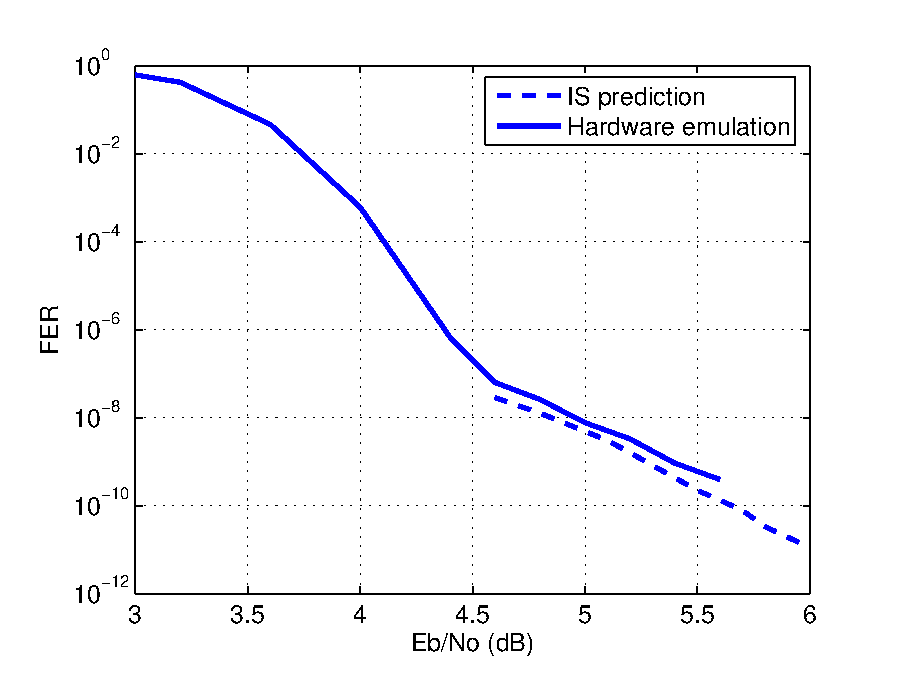
\includegraphics[width=2.8in,height=2.1in]{itwfig6_0619.eps}
\caption{Mean-shift IS bound and hardware results: 6-bit decoder.
}\label{exp1}
\end{figure}
\begin{figure}
\vspace{0.0in}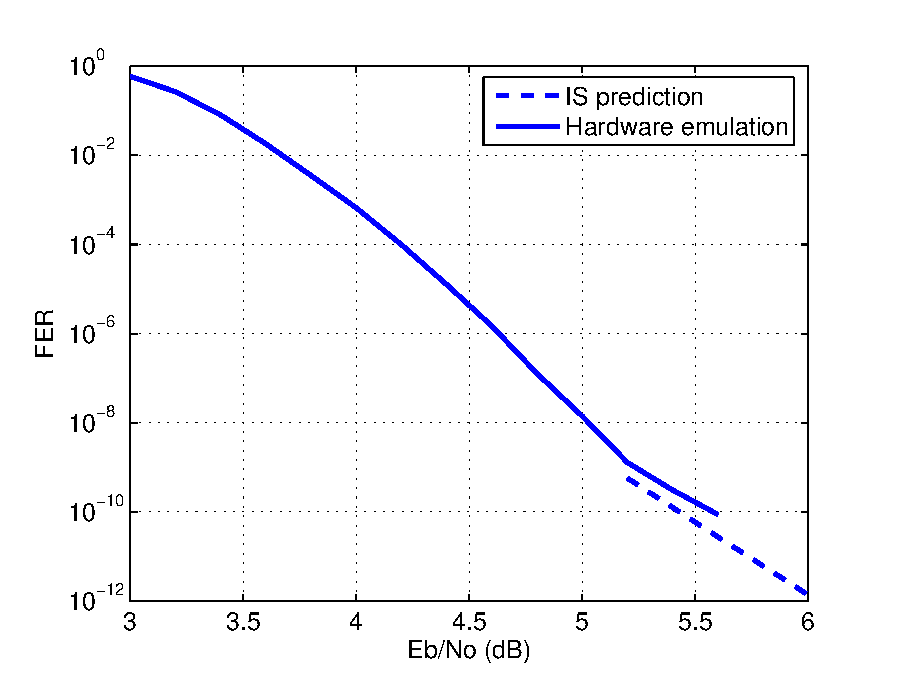
\includegraphics[width=2.8in,height=2.1in]{itwfig7_0619.eps}
\caption{Mean-shift IS bound and hardware results: 9-bit decoder.
}\label{exp2}
\end{figure}

\begin{figure}\center\begin{tabular}{|c|c|c|c|c|}
  \hline
  % after \\: \hline or \cline{col1-col2} \cline{col3-col4} ...
  SNR & Sample Variance & Simulation Gain \\
  \hline
  4.6 &  9.64E-25 & 4.6E6 \\
  4.8 &  2.29E-26 & 1.9E7 \\
  5.0 &  3.29E-27 & 2.77E7 \\
  5.2 &  1.18E-28 & 7.58E8 \\
  \hline
\end{tabular}
\caption{Simulation gains for the 6-bit decoder based on
mean-shift}\label{table11}
\end{figure}

\begin{figure}\center\begin{tabular}{|c|c|c|c|c|}
  \hline
  % after \\: \hline or \cline{col1-col2} \cline{col3-col4} ...
  SNR &  Sample Variance & Simulation Gain \\
  \hline
  5.2 & 3.7E-28 & 4.0E8 \\
  5.4 & 4.4E-29 & 6.72E8 \\
  5.6 & 4.07E-31 & 3.12E9 \\
  \hline
\end{tabular}
\caption{Simulation gains for the 9-bit decoder based on the
mean-shift.}\label{table12}
\end{figure}



 The above results demonstrate that even a
simple prediction is useful in estimating the performance of a
code in the low FER region. %For both quantization choices, the
%predicted importance sampling based curve provides an approximate
% bound on the probability of error that is within a factor of 10
%of the hardware based simulation results.
Moreover, since the
simulation gain increases with the increase in SNR, the
computational benefits of using the proposed importance sampling
based prediction increases with increased SNR/lower FER.

%\vspace{1in} MISSING POINT 3: DISCUSSION OF 6-BIT VS 9-BIT
%DECODING REGION

We now discuss the effects of the implementation choices on the
decoding region. As observed from Figures~\ref{exp1} and~\ref{exp2},
the error floor improves from a 6-bit decoder implementation to a
9-bit decoder implementation in hardware emulations. These additional
3 bits permit more quantization levels to better distinguish messages
during the message passing. Specifically, the soft messages in this
6-bit decoder suffer from more severe message saturations (clipping)
than in its 9-bit decoder counterpart. In the high-SNR error floor
regime, the clipping effect is more pronounced on strong ``good''
messages. These good messages do not have a strong enough
representation, thereby leading to an absorbing state where good
messages can be overcome by the sheer number of bad messages. As a
result, the decoder is more easily pulled into the absorbing state
under the 6-bit quantization than under the 9-bit quantization. This
effect can be also seen from the observation that under the same mean
shift, the relative number of errors for the 6-bit quantization scheme
is uniformly higher than for the 9-bit scheme, as seen by comparing
Tables~\ref{tab1} and~\ref{tab4}. (Note that both simulations are
based on $N = 10^4$ trials at SNR $5.4$ dB.)
% This intuition is also confirmed by hardware emulations of a 6-bit
%decoder, in which we observed a stronger tendency towards the
%absorbing state compared to a 9-bit
%decoder. %MISSING PT 3: CONNECTION TO THE DECODING REGION
%We thus conjecture that with the help of a relatively small mean
%shift, this tendency can be accentuated, causing absorbing-set
%errors. Accordingly, the convergence region of an absorbing set in
%a 6-bit decoder is larger than the convergence region of a 9-bit
%decoder.

\begin{figure}\center\begin{tabular}{|c|c|c|c|c|}
  \hline
  % after \\: \hline or \cline{col1-col2} \cline{col3-col4} ...
  Mean Shift & Ratio  \\
  \hline
  0.8 &   0.0060\\
  1.0 &   0.1002\\
  1.2 &   0.4944\\
  1.6 &   0.9890\\
  \hline
\end{tabular}
\caption{Ratio of absorbing set errors and total number of trials
for the 9-bit decoder.}\label{tab4}
\end{figure}
\section{Concluding Remarks}\label{conc}

LDPC codes have recently generated a lot of interest due to their
excellent performance. While the infinite blocklength regime is better
understood, less is known about the performance of LDPC codes for
finite blocklengths. Since the performance of finite blocklength LDPC
codes for low FER rates cannot be estimated reasonably fast using
software based Monte Carlo simulations, along with the lack of
finite-length theoretical analysis, the deployment of LDPC has so far
been somewhat limited.

In this paper, we presented a technique for estimating probability of
decoding error of LDPC codes in the low FER/BER regime. The proposed
method utilizes importance sampling to quickly produce the estimate of
the performance. With appropriately biased densities, the runtime
speed-up is on the order of millions. In conjunction with the
description and count of dominant absorbing errors, the proposed
technique provides accurate estimates of the probability of error in
the low FER regime. Results obtained on a hardware emulator are
consistent with the proposed technique, and thus suggest the promise
of using the proposed approach at even lower FER/BER levels.

As to future directions, we plan to extend the proposed methodology to
other LDPC codes with different absorbing set configurations and their
distributions as well as to investigate how the decoding regions
associated with the codewords and the absorbing sets scale as a
function of the decoder choices, specifically including the min-sum
algorithm as a less complex version of the message passing decoding.
